\chapter{Surface Simulations results}
\label{chap:ehd_res}

\section{Post-processing}

Fig. \ref{ch5:fig:activeness_map} show how {\tdsim} can be used to generate an activeness map for a detector. This map is produced by simulating about 100 points coarsely spaced through the detector and then interpolated using cubic interpolation. These maps can then be used with Monte Carlo background estimation methods to create energy spectrum for surface events for experiments such as LEGEND


-trap filter
-mapping the detector
-interpolation

\begin{figure}[!htb]
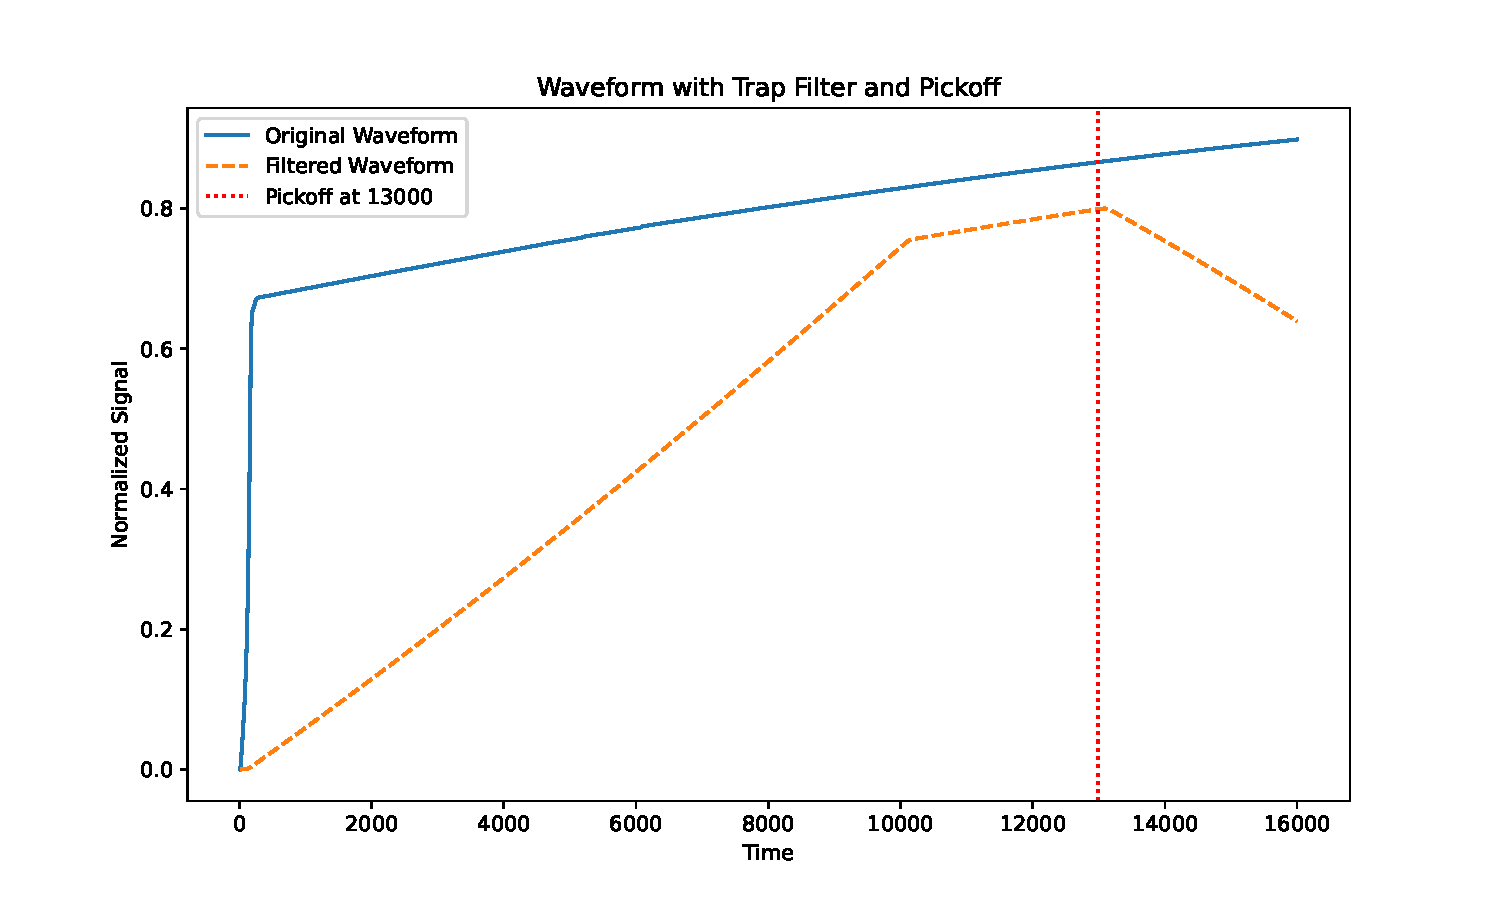
\includegraphics[trim={0cm 0cm 0cm 0cm},clip,width=\linewidth]{ch5/figs/trap_filt.pdf}
\caption{Sample trap filter}
\label{ch5:fig:trap_filter}
\end{figure}

\begin{figure}
%[trim={left bottom right top},clip]

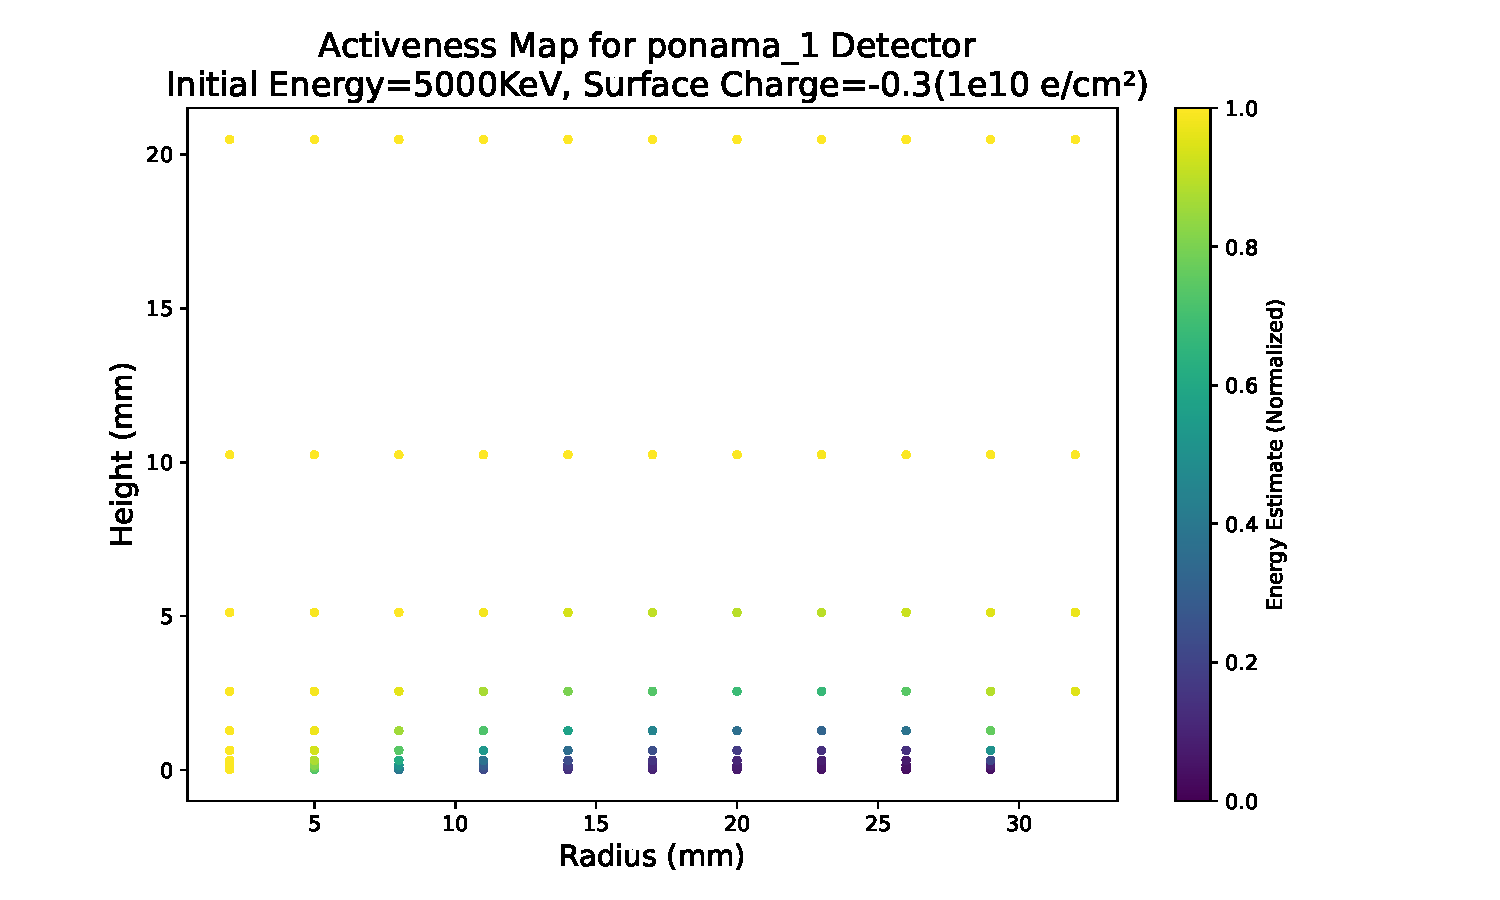
\includegraphics[trim={0cm 0.5cm 3.2cm 1.15cm},clip,width=\linewidth]{ch5/figs/activenss_map_ponama_1_-0.3.pdf}
\caption{Activeness map for a PPC detector \tdsim with initial energy 5000 keV and s}
\label{ch5:fig:activeness_map}
\end{figure}


\begin{figure}
%[trim={left bottom right top},clip]
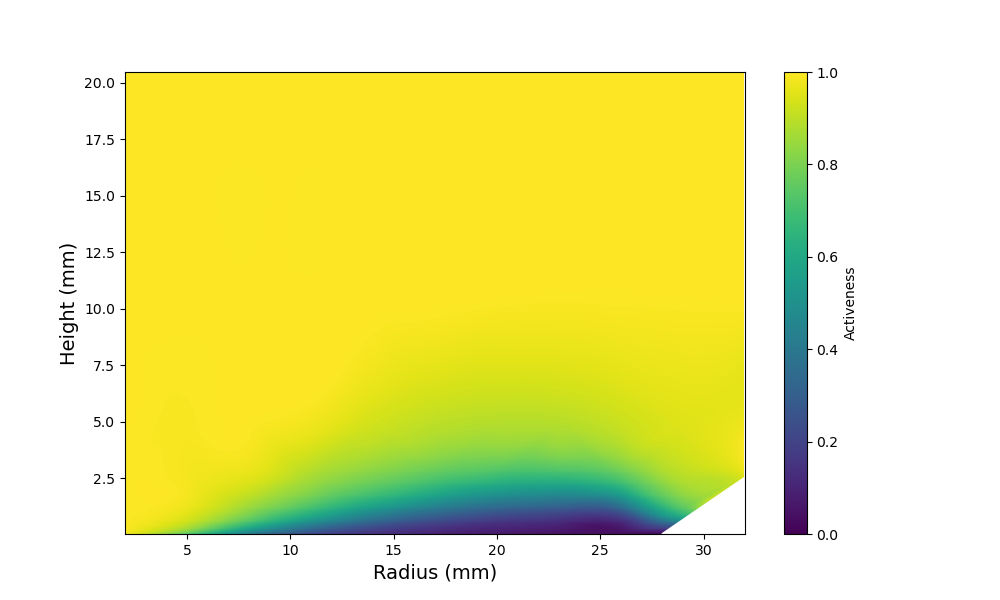
\includegraphics[trim={1.4cm 0.5cm 3.2cm 1.755cm},clip,width=\linewidth]{ch5/figs/activeness_map_cubic_sc=-0.3_ponama_1_5000.png}
\caption{Interpolated Activeness map for a PPC detector \tdsim}
\label{ch5:fig:interpolated_activeness_map}
\end{figure}

\begin{figure}
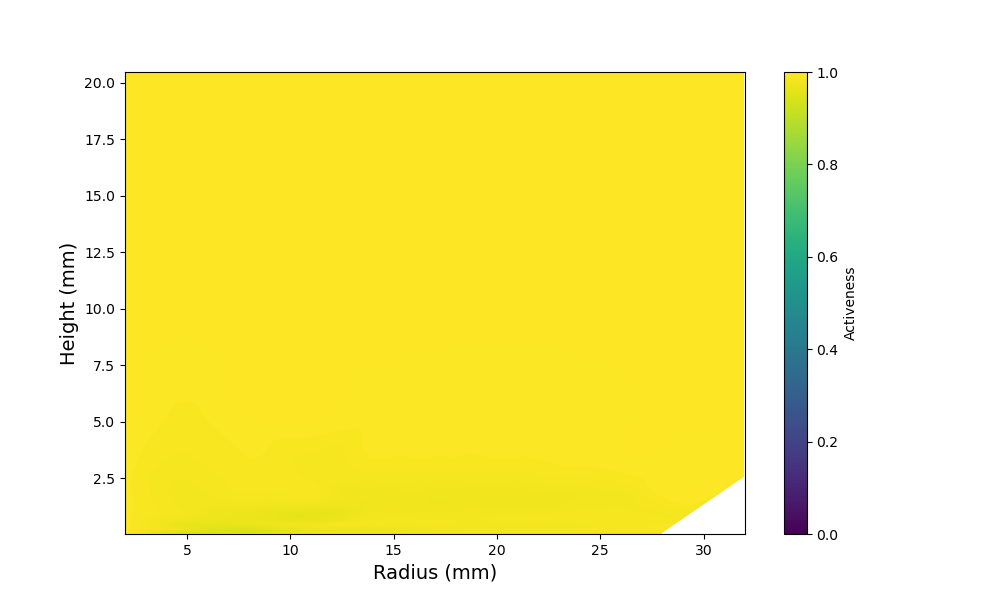
\includegraphics[trim={1.5cm 0cm 3.3cm 1cm},clip,width=0.49\linewidth]{ch5/figs/activeness_map_cubic_sc=0_ponama_1_5000.png}
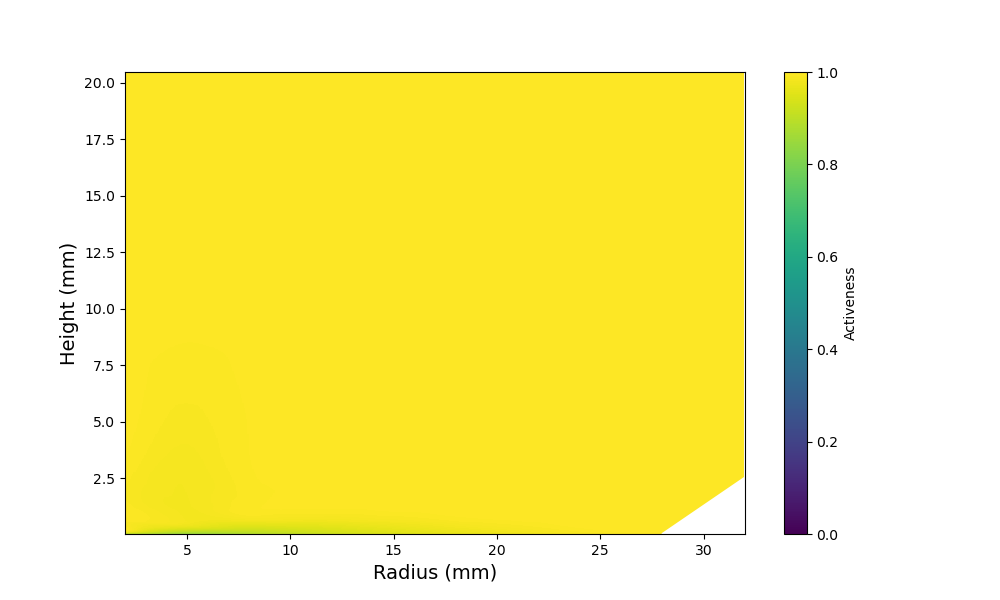
\includegraphics[trim={1.5cm 0cm 3.3cm 1cm},clip,width=0.49\linewidth]{ch5/figs/activeness_map_cubic_sc=0.3_ponama_1_5000.png}
\caption{Interpolated Activeness map for a PPC detector \tdsim for 0 and positive surface charge}
\label{ch5:fig:interpolated_activeness_map_0_pos}
\end{figure}


\section{\label{res:1} Reproducing results from know test stands}


To validate EH-Drift against existing measurements, we modeled alpha events studied by two separate scanning test stands known as TUBE\cite{tube_paper} and GALATEA\cite{galatea_paper}. These scanners yielded conflicting dependencies of collected energy on radial position. TUBE reported that energy increased with radius, whereas GALATEA reported the opposite trend. We simulated each scanner’s geometry and tested various values of surface charge and surface-to-bulk drift ratios. 

We simulated events for detector used in those scanner using various surface charges. We generated 8$\mu$s pulse using {\tdsim} and applied a trap filter of 4$\mu$s rise time, 3$\mu$s flat top time and picked off energy at 7$\mu$s. We then fit the data using various surface charge to estimate the amount of surface charge present to show such behavior.


\begin{figure}
%[trim={left bottom right top},clip]

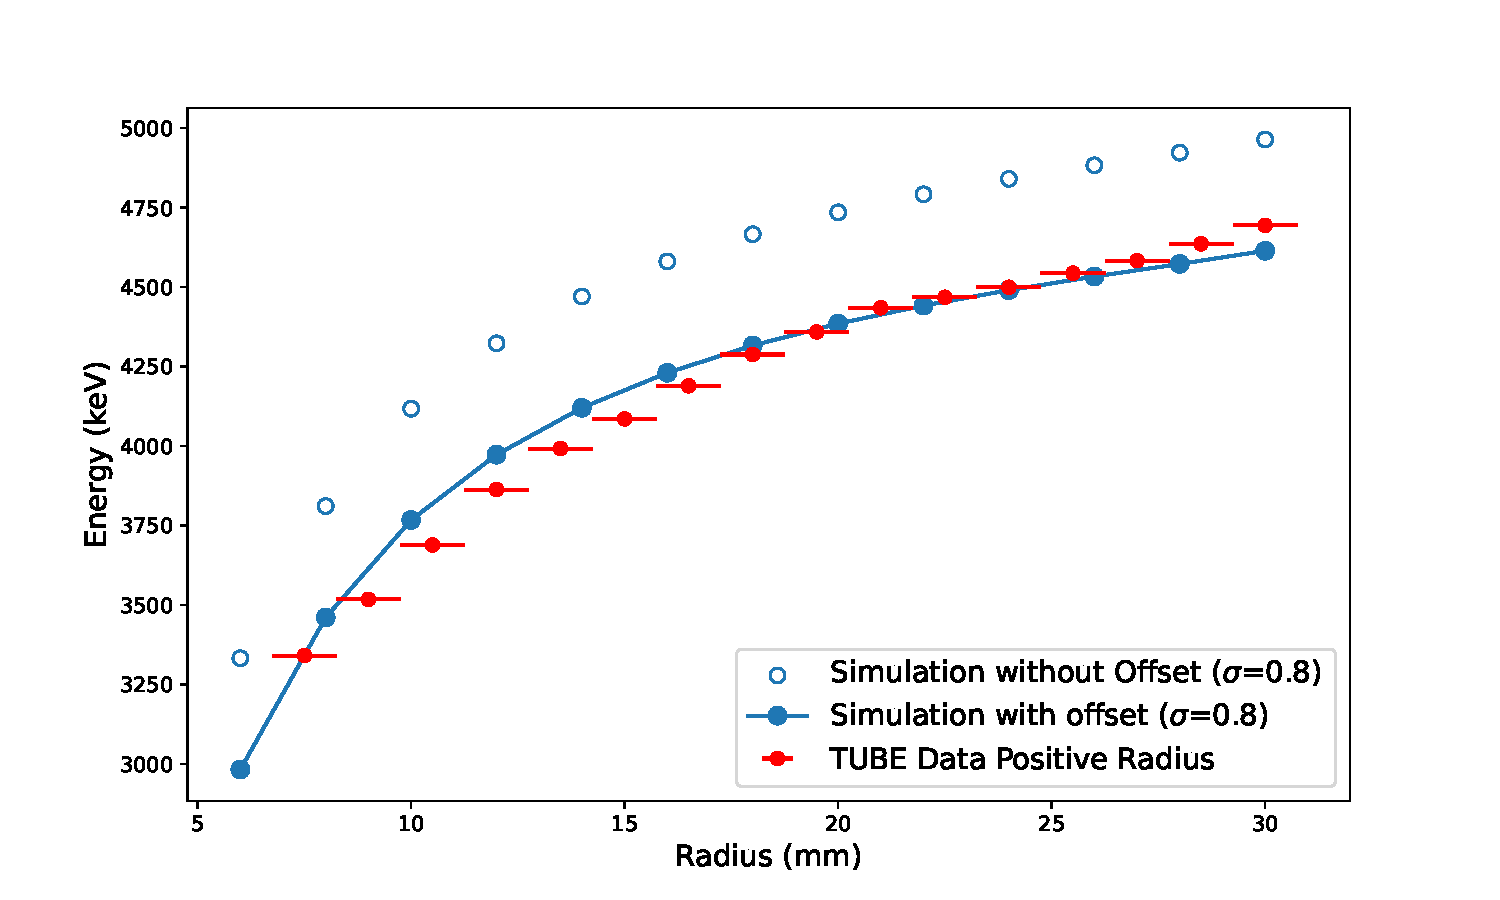
\includegraphics[trim={0.3cm 0.1cm 1.7cm 0.1cm},clip,width=\linewidth]{ch5/figs/tube_fit.pdf}
\caption{Fitting the activeness in TUBE scanner with \tdsim{}.}
\label{fig:tube_fit}
\end{figure}


\begin{figure}
%[trim={left bottom right top},clip]

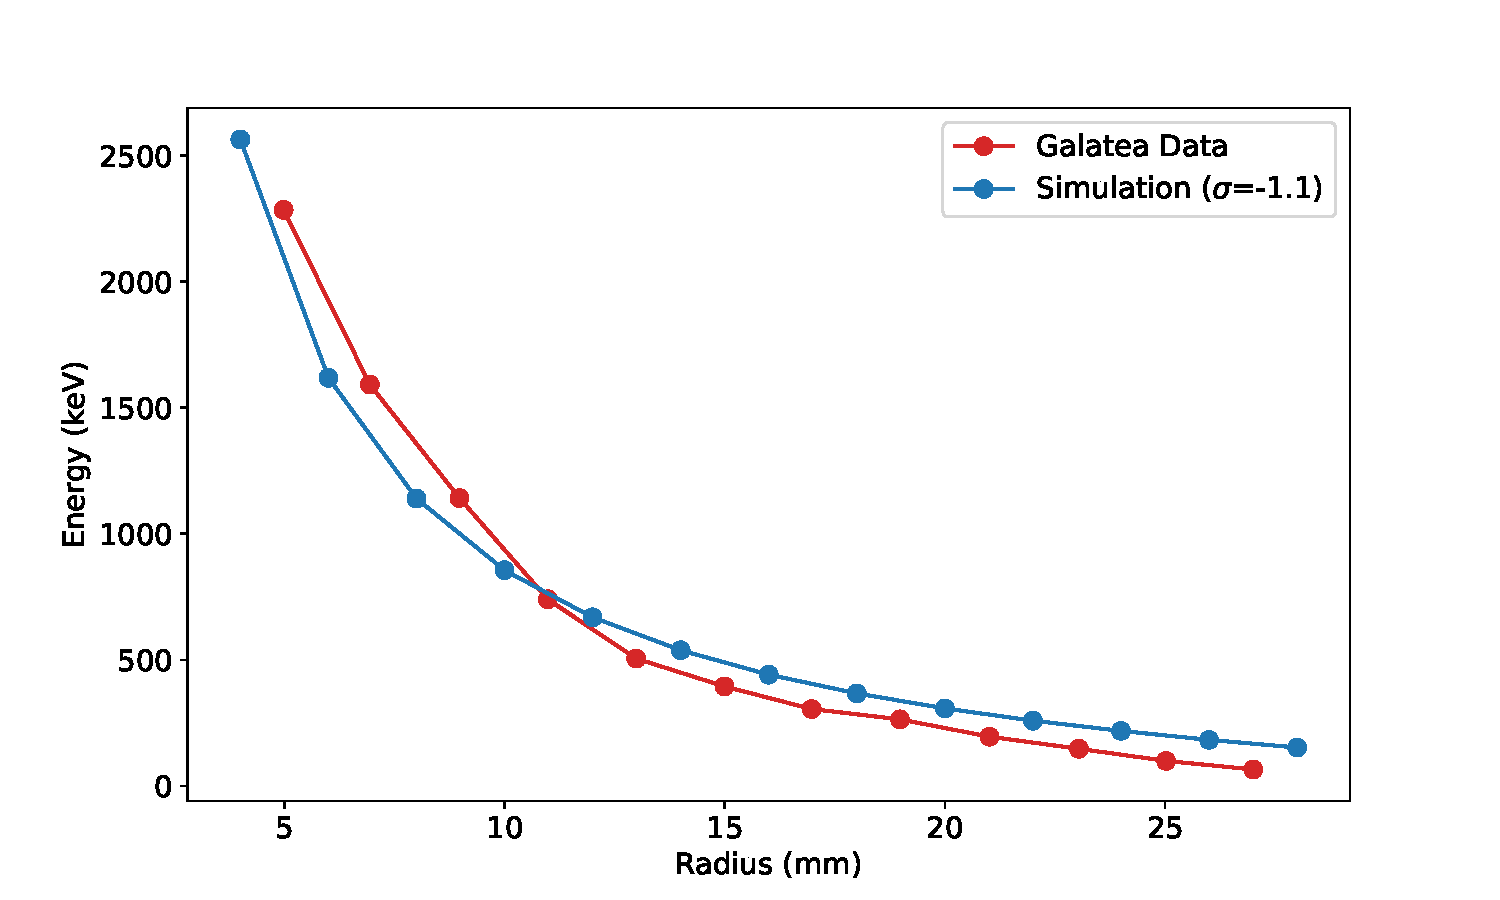
\includegraphics[trim={0.3cm 0.1cm 1.7cm 0.1cm},clip,width=\linewidth]{ch5/figs/gal_fit.pdf}
\caption{Fitting the activeness in GALATEA scanner with \tdsim{}.}
\label{fig:gal_fit}
\end{figure}

We found a positive surface charge explains the behavior observed in TUBE. Fig. \ref{fig:tube_fit} compares TUBE scanner data to EH-Drift simulations with a positive surface charge Positive surface charge would attract electrons on the surface which would result in energy degradation. In this scenario, electrons are collected at the n+ surface, so closer the points are to the origin, more chance there is for the electrons to get trap onto the surface, and more energy degradation there is. Thus collected energy is proportional to radius.



In the GALATEA scanner, the behavior can be explained using a negative surface charge as shown in Fig. \ref{fig:gal_fit}. Negative surface attracts hole to the surface and since holes are collected at point contact, located at r=0, the higher the radius, more charges end up on the surface. Thus collected energy fall inversely with radius.

-add maps for positive and zero surface charges



\section{\label{res:2} Estimating efficiency in ROI}


We can use the maps created by EH to estimate the collections efficiency of signature events such as {\onbb}. Experiemnts such as Legend have a region of interest (ROI) band determined by the energy resolutions of the detector. ROI is used to clasify if an event is signature event or not; however if the event happens close to the surface, there is a chance that the collected energy would be degraded enough to not register as an event in ROI. To understand this effect we created activeness maps for detectors with 2039 keV initial energy for various surface charges. We then randomly sample points uniformly in the detector and estimate their activeness using the interpolated map. A 3 keV threshold is defined for the Region of Interest (ROI), meaning that if the activeness at a point falls below 3 keV, that event is not registered as a {\onbb} event. Each point is assigned a value of 1 if it is counted as {\onbb}, or 0 otherwise. The overall efficiency is then calculated as the sum of activeness values divided by the total number of points, while also factoring in the phi dependence.

Fig. \ref{fig:efficiency_sc_plot} shows the estimated efficiency versus surface charge for the {\ponama} detector, a LEGEND PPC detector, and a LEGEND ICPC detector. The efficiency drops rapidly for negative surface charges in both PPC detectors; however, it decreases most sharply for {\ponama}, which has a lower depletion voltage and thus a weaker electric field near the surface. The LEGEND PPC detector also loses efficiency quickly because of its larger passivated surface, but its higher electric field moderates the overall loss more than in {\ponama}. Finally, the Mirion-style ICPC detector exhibits virtually no reduction in activeness, primarily because it has a much smaller passivation region. Since LEGEND-1000 plans to use Mirion-style ICPC detectors, surface backgrounds in that experiment are expected to be significantly reduced.

\begin{figure}[!htb]
\centering
%[trim={left bottom right top},clip]
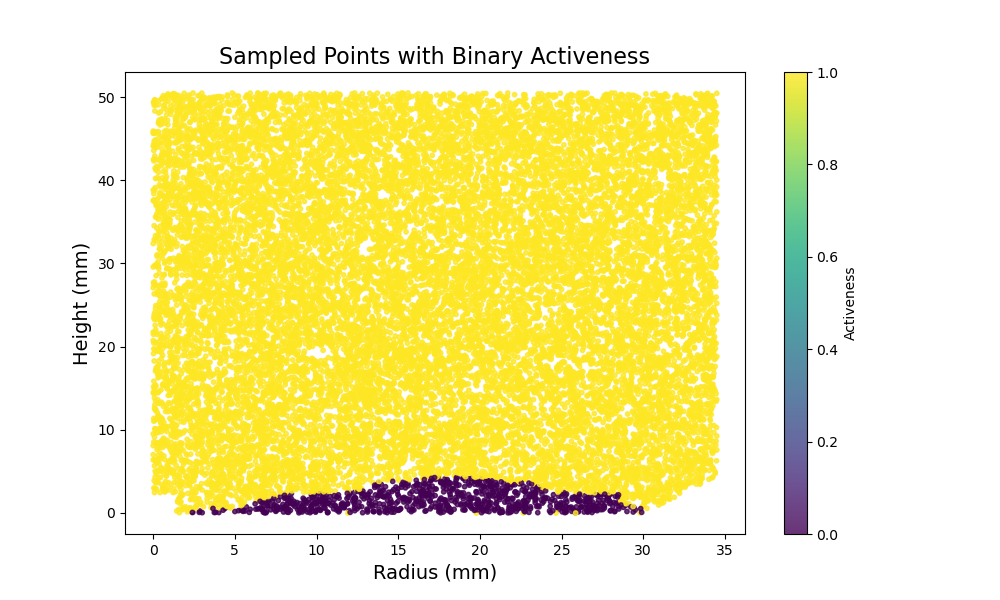
\includegraphics[trim={1.5cm 0cm 6cm 0cm},clip,width=0.9\linewidth]{ch5/figs/bianry_act_ponama_1_-0.03.png}
\caption{Binary activeness.}
\label{ch5:fig:binary_activenss}
\end{figure}

\begin{figure}[!htb]
%[trim={left bottom right top},clip]
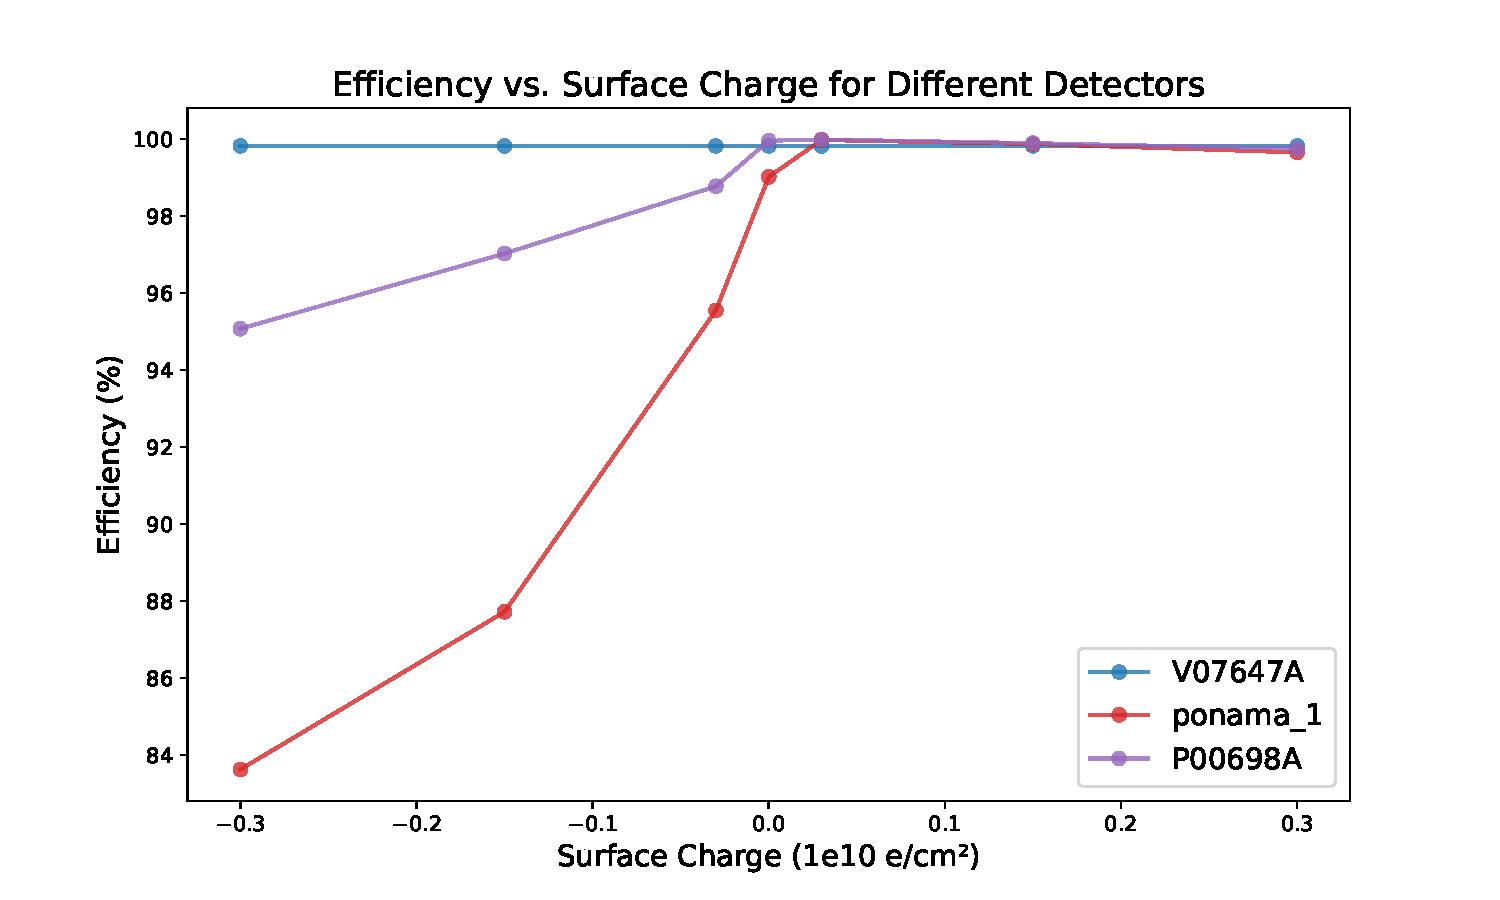
\includegraphics[trim={1.6cm 0.3cm 2cm 1.8cm},clip,width=\linewidth]{ch5/figs/efficiency_0nbb.pdf}
\caption{Efficiency in the ROI versus surface charge.}
\label{fig:efficiency_sc_plot}
\end{figure}

\begin{figure}
%[trim={left bottom right top},clip]
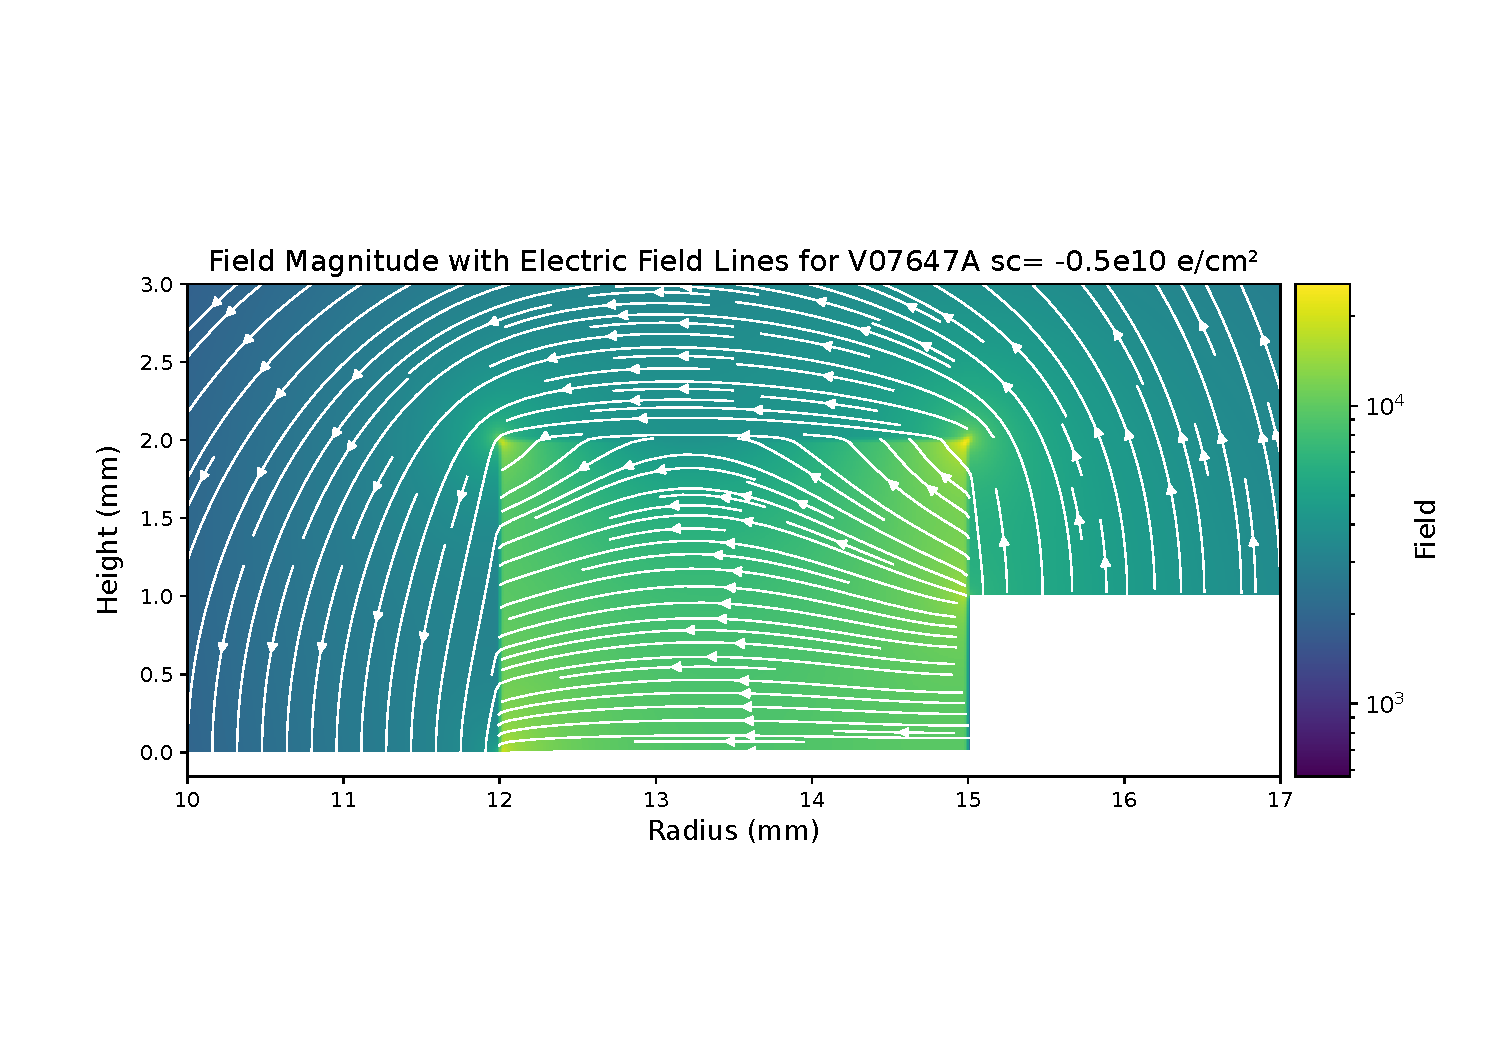
\includegraphics[trim={0cm 4cm 0cm 4cm},clip,width=0.99\linewidth]{ch5/figs/elect_field_lines_surface_V07647A_sc_-0.5.pdf}
\caption{Electric field lines near the ditch of the detector.}
\label{ch5:fig:elect_field_lines_surface_V07647A}
\end{figure}
\section{\label{res:3} Generating Background Spectra}

To demonstrate how EH-Drift can be used to create a background model, we performed a Geant4 simulation of a germanium detector exposed to a planar 5\,MeV alpha source. We recorded the resulting hits from alpha particles entering the detector. We then used the activeness map to estimate the energy that would be collected due to surface effect. Fig. \ref{fig:eng_spec_degradation} how the collected energy spectrum would look like for various surface charge scenarios. Notably, the spectrum for negative surface charge closely matches alpha spectra estimated in experimental data.

\begin{figure}[!htb]
  \centering
      %[trim={left bottom right top},clip]

  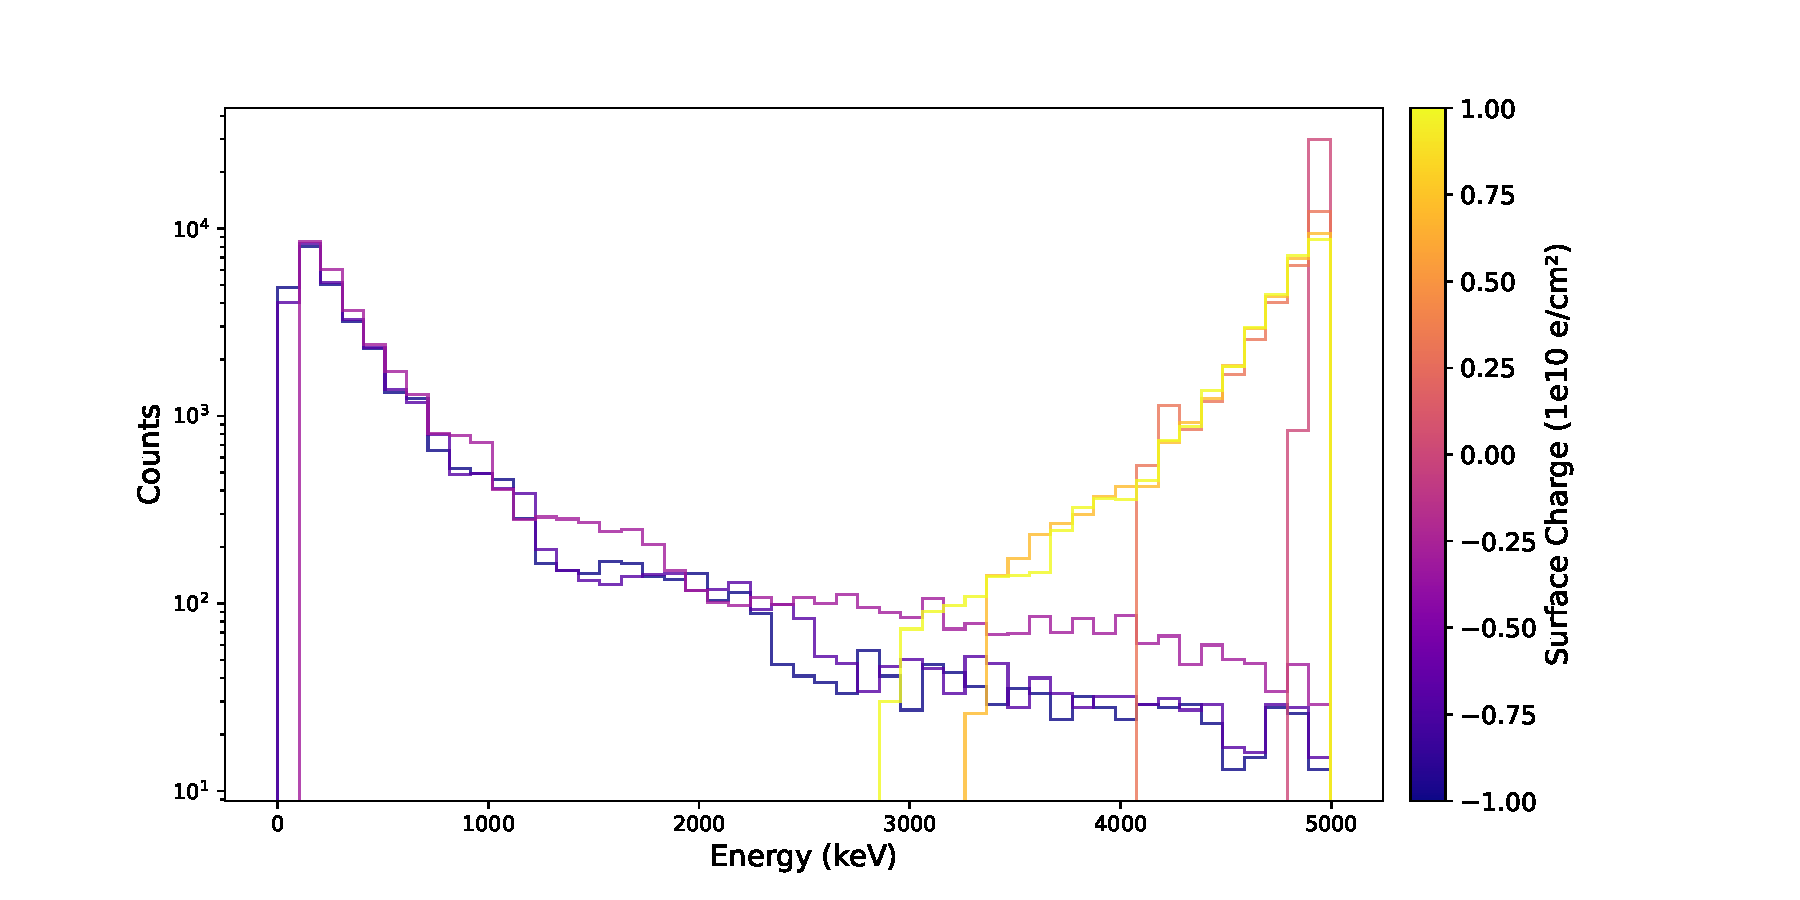
\includegraphics[trim={2cm 0.5cm 4.5cm 1.7cm},clip,width=0.99\linewidth]{ch5/figs/eng_deg_hist.pdf}
  \caption{Degradation of the alpha-particle energy spectrum under various surface charges. The initial alpha energy was 5\,MeV.}
  \label{fig:eng_spec_degradation}
\end{figure}


\begin{figure}[!htb]
  \centering
      %[trim={left bottom right top},clip]
  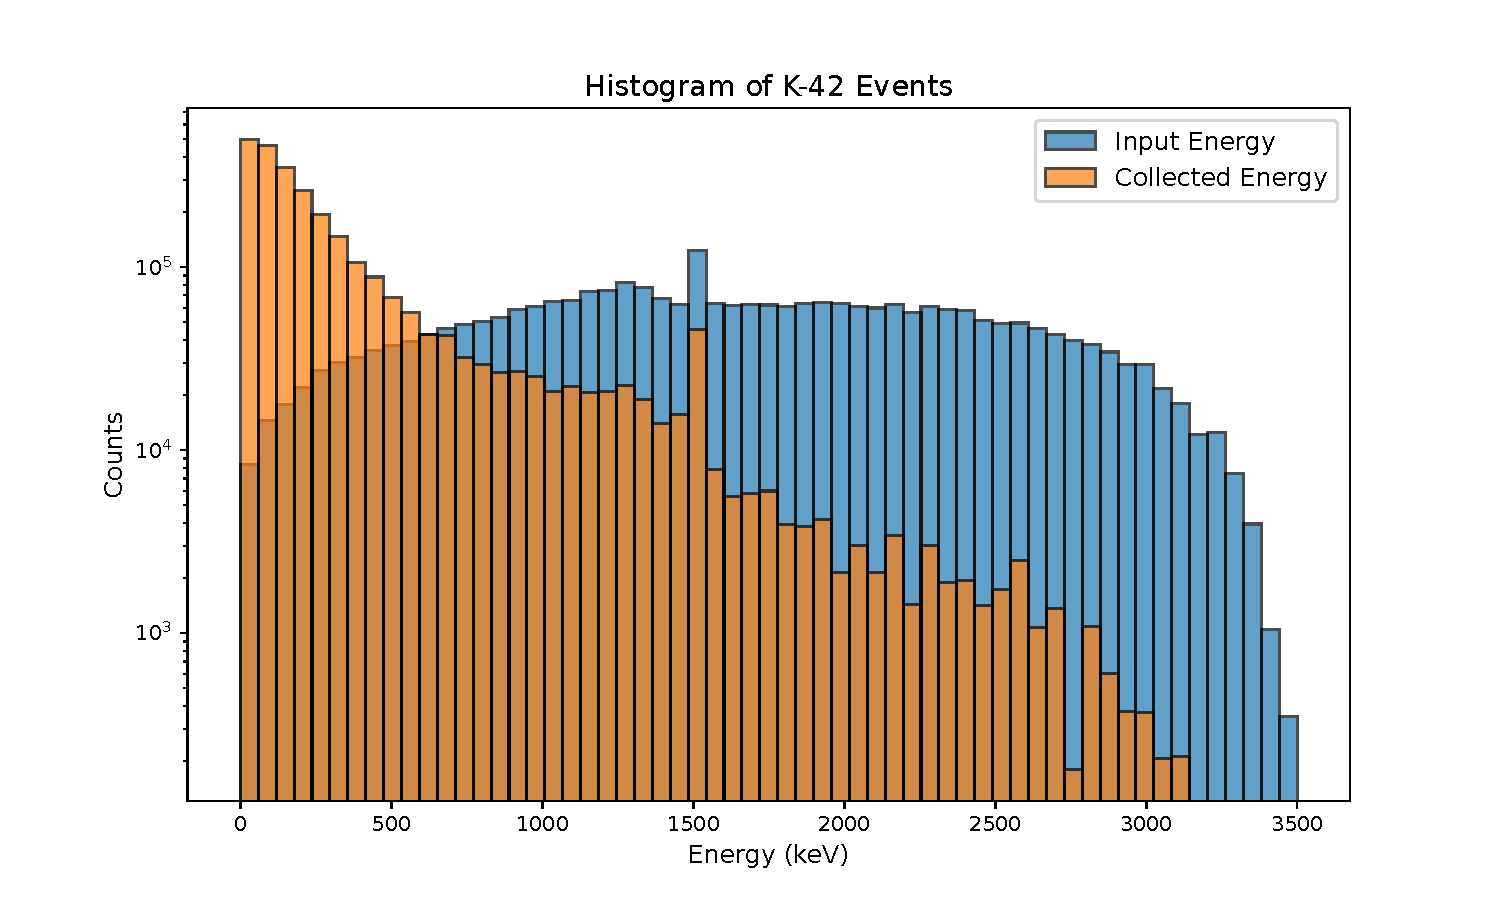
\includegraphics[trim={1.5cm 0.0cm 2cm 0cm},clip,width=0.99\linewidth]{ch5/figs/k_42_beta_spectrum.pdf}
  \caption{Degradation of the }
  \label{ch5:figs:k_42_degrad}
\end{figure}




\section{Conclusion}
EH-Drift extends the capabilities of existing HPGe detector simulations by incorporating detailed physical processes such as diffusion, self-repulsion, and surface charge effects, all while maintaining computational efficiency through GPU acceleration. Its ability to model large charge cloud drifts and surface drifts makes it a valuable tool for understanding detector response to surface events and improving background modeling in experiments.
